\synctex=1
\documentclass[11pt, a4paper]{article}

%% Packages
\usepackage{subcaption}
\usepackage{amsthm}
\usepackage{amsmath}
\usepackage{amsfonts}
\usepackage{booktabs}
\usepackage{natbib}
\usepackage{hyperref}
% \usepackage{fullpage}
\usepackage{graphicx}
\usepackage{mathtools}
\usepackage{color}
\usepackage[left = 2.5cm, right = 2.5cm, bottom = 3cm, top = 2.5cm]{geometry}
% \usepackage{enumitem}
\usepackage{multirow}
\usepackage{rotating}
\usepackage{calc}
\usepackage{bm}
\usepackage{pdfpages}
\usepackage{authblk}
\usepackage{dcolumn}
\usepackage{float}


\usepackage[inline]{showlabels}
\renewcommand{\showlabelfont}{\small\tt\color{red}}

%% Commands 
% \newcommand*{\bb}{}
\newcommand*{\bb}{\boldsymbol}
\newcommand{\IK}[1]{{\noindent \color{blue} \bf \#IK: #1}}
\newcommand{\PS}[1]{{\noindent \color{red} \bf \#PS: #1}}
\newcommand{\iq}[3]{#1^{#2}_{#3}}
\newcommand{\mi}[5]{\prescript{#3}{#2}{{#1}}_{#4}^{#5}}
\newcommand{\Q}[4]{\tilde Q_{#1}^{(#2,#3,#4)}}
\newcommand{\pQ}[4]{Q_{#1}^{(#2,#3,#4)}}
\newcommand{\Op}[1]{\ensuremath{{\mathcal{O}_p(#1)}}}
\newcommand{\op}[1]{\ensuremath{{o_p(#1)}}}


\newcommand{\vnorm}[1]{\ensuremath{{\left\| #1 \right\|}}}
\newcommand{\mnorm}[1]{{\left\vert\kern-0.25ex\left\vert\kern-0.25ex\left\vert #1 
		\right\vert\kern-0.25ex\right\vert\kern-0.25ex\right\vert}}
\newcommand{\mnorms}[1]{{\vert\kern-0.25ex\vert\kern-0.25ex\vert #1 
		\vert\kern-0.25ex\vert\kern-0.25ex\vert}}

       
%% Theorems etc
\newtheoremstyle{example}% name
{3pt} %Space above
{3pt} %Space below
{} %Body font
{0\parindent} %Indent amount 1
{\bf}
% {\scshape} %Theorem head font
{:} %Punctuation after theorem head
{.5em} %Space after theorem head 2
{} %Theorem head spec (
\newtheoremstyle{theorem}% name
{3pt} %Space above
{3pt} %Space below
{\em} %Body font
{0\parindent} %Indent amount 1
{\bf}
% {\scshape} %Theorem head font
{:} %Punctuation after theorem head
{.5em} %Space after theorem head 2
{} %Theorem head spec (
\theoremstyle{example} \newtheorem{example}{Example}[section]
\theoremstyle{theorem} \newtheorem{theorem}{Theorem}[section]
\newtheorem*{proposition}{Proposition}
\newtheorem{lemma}[theorem]{Lemma}


%% Definitions
\def\sign{\mathop{\rm sign}}
\def\expect{{\mathop{\rm E}}}
\def\var{{\mathop{\rm var}}}
\def\cov{{\mathop{\rm cov}}}
\def\trace{{\mathop{\rm trace}}}
\def\det{{\mathop{\rm det}}}

\def\bbeta{\bb{\beta}}
\def\btheta{\bb{\theta}}
\def\bpsi{\bb{\psi}}
\def\bgamma{\bb{\gamma}}
\def\bSigma{\bb{\Sigma}}
\def\bgamma{\bb{\gamma}}
\def\by{\bb{y}}
\def\bC{\bb{C}}
\def\bY{\bb{Y}}
\def\bu{\bb{u}}
\def\bx{\bb{x}}
\def\bz{\bb{z}}
\def\b0{\bb{0}}
\def\bX{\bb{X}}
\def\bZ{\bb{Z}}
\def\bv{\bb{v}}
\def\bV{\bb{V}}
\def\bY{\bb{Y}}
\def\by{\bb{y}}
\def\bL{\bb{L}}
\def\bLt{\tilde{\bb{L}}}
\def\btnod{\bb{\theta}_0}
\def\bttilde{\tilde{\bb{\theta}}}
\def\bW {\bb{W}}
%% Title Page 
\title{Maximum softly-penalized likelihood for mixed effects logistic regression}
 
\author[1]{Philipp Sterzinger}
\author[1,2]{Ioannis Kosmidis}

\affil[1]{Department of Statistics, University of Warwick, Coventry, CV4 7AL, UK}
\affil[2]{The Alan Turing Institute, London, NW1 2DB, UK}

\begin{document}
\maketitle
%\tableofcontents

\begin{abstract}
Maximum likelihood estimation in logistic regression with mixed
effects is known to have a positive probability to result in
estimates on the boundary of the parameter space. Such estimates,
which include infinite values for fixed effects and singular or
infinite variance components, can cause havoc to numerical
estimation procedures and inference. We introduce an additive
penalty to the log-likelihood function, or an approximation thereof,
which consists of appropriately scaled versions of the Jeffreys'
prior for the model with no random effects and of a composition of
the negative Huber loss for the variance components. The resulting
maximum penalized likelihood estimates are shown to lie in the
interior of the parameter space. Appropriate scaling of the penalty
guarantees that the penalization is soft enough to preserve the
optimal asymptotic properties expected by the maximum likelihood
estimator, namely consistency, asymptotic normality, and
Cram\'{e}r-Rao efficiency. Our choice of penalties and scaling
factor preserves equivariance of the fixed effects estimates under
linear transformation of the model parameters, such as
contrasts. Maximum softly-penalized likelihood is compared to
competing approaches on two real-data examples, and through
comprehensive simulation studies that illustrate its superior finite
sample performance.
  \bigskip \\
  \noindent {Keywords: logistic regression, infinite estimates, singular variance components, data separation, Jeffreys' prior}
\end{abstract}

\section{Introduction}
\label{sec:intro}

Generalized Linear Mixed Models (GLMMs; \citealt[Chapter
7]{mcculloch+etal:2008}) are a potent class of statistical models that
can associate Gaussian and non-Gaussian responses, such as counts,
proportions, positive responses, and so on, with covariates, while
accounting for complex multivariate dependencies. This is achieved by
linking the expectation of a response to a linear combination of
covariates and parameters (fixed effects), and sources of extra
variation (random effects) with known distributions. Although these
models find application in numerous fields such as biology, ecology
and the social sciences \citep{bolker+etal:2009}, estimation of GLMMs
is not straightforward in practice because their likelihood is
generally an intractable integral.

Maximum likelihood (ML) methods for GLMMs maximize the GLMM likelihood or
an approximation thereof, that can in principle be made
arbitrarily accurate \citep[see, for example,
][]{raudenbush+etal:2000, pinheiro+chao:2006}. Such methods are
pervasive in contemporary GLMM practice because the resulting
estimators are consistent under general model regularity conditions,
and the resulting estimates and the (approximate) likelihood can be used for
 likelihood-based inferential devices, such as
likelihood-ratio or Wald tests, and model selection procedures based
on information criteria. An alternative approach is to use Bayesian
posterior update procedures \citep[see, for
example,][]{zhao+etal:2006,browne+draper:2006}. However, such
procedures come with various technical difficulties, such as
determining the scaling of the covariates, selecting appropriate
priors, coming up with efficient posterior sampling algorithms, and
determining burn-in times of chains for reliable estimation. Yet
another alternative are maximum penalized
quasi-likelihood methods \citep{schall:1991, wolfinger+oconnel:1993,
  breslow+clayton:1993} which essentially fit a linear mixed model to
transformed pseudo-responses. However, the penalized quasi-likelihood
may not yield an accurate approximation of the GLMM likelihood. As a
result, these estimators can have large bias when the random
effects variances are large
\citep{bolker+etal:2009,rodriguez+goldman1995} and are not necessarily
consistent \citep[Chapter 3.1]{jiang:2017}.

Despite the pervasiveness of ML methods in the statistical of GLMMs,
certain data configurations can result in estimates of the
variance-covariance matrix of the random effects distribution to be on
the boundary of the parameter space, such as infinite or zero
estimated variances, or, more generally, singular estimates of the
variance-covariance matrix; see \citet[Section 2.1]{chung+etal:2013}
for an excellent discussion. In addition, as is the case in ML
estimation of Bernoulli-response generalized linear models
\citep[GLMs; see, for example][Chapter 4]{mccullagh+nelder:1989}, the
ML estimates of the fixed effects for GLMMs can be infinite. As is
well-acknowledged in the GLMM literature \citep[see, for
example][]{bolker+etal:2009, bolker:2018, pasch+etal:2013}, both
instances of boundary estimates can cause havoc to numerical
optimization procedures, and if boundary estimates go undetected, they
may substantially impact first-order inferential procedures, like Wald
tests, resulting in spuriously strong or weak conclusions. In contrast
to the numerous approaches to detect (see, for example,
\citealt{kosmidis+schumacher:2021} for the \texttt{detectseparation} R
\citep{R} package that implements the methods in \citealt{konis:2017})
and handle \citep[see, for example,][]{kosmidis+firth:2021,
  heinze+schemper:2002, gelman+etal:2008} infinite estimates in
logistic regression with fixed effects, little methodology or guidance
is available on how to detect or deal with degenerate estimates in
logistic regression with mixed effects. For this reason, it is
practically desirable to have access to methods that are guaranteed to
return estimates away from the boundary of the parameter space, while
preserving the key properties that the maximum likelihood estimator
has.

We introduce a maximum softly-penalized (approximate) likelihood
(MSPL) procedure for mixed effects logistic regression that returns
estimators that are guaranteed to take values in the interior of the
parameter space, and are also consistent, asymptotically normal, and
Cram\'{e}r-Rao efficient, under the assumptions typically employed for
establishing consistency, and asymptotic normality of ML
estimators. The penalty we propose consists of appropriately scaled
versions of Jeffreys' invariant prior for the model with no random
effects, and of compositions of the negative Huber loss functions for
the variance components. We show that the MSPL estimates are
guaranteed to be in the interior of the parameter space, and scale the
penalty appropriately to guarantee that i) penalization is soft enough
for the MSPL estimator to have the same optimal asymptotic properties
expected by the ML estimator, and ii) that the fixed effects estimates
are equivariant to linear transformation of the model parameters, such
as contrasts, in the sense that the MSPL estimates of linear
transformations of the fixed effects parameters are the linear
transformations of the MSPL estimates. Both i) and ii) are in contrast
to other prominent penalization procedures \citep[see, for
example,][]{chung+etal:2013, chung+etal:2015}, for which open-source
software implementations exist (for example, the \texttt{bglmer}
routine of the \texttt{blme} R package). Maximum softly-penalized
likelihood is compared to prominent competing approaches through two
real-data examples and comprehensive simulation studies that
illustrate its superior finite-sample performance. Although the
developments here are for logistic regression with mixed effects, they
provide a blueprint for the construction of penalties and estimators
of the fixed effects and/or the variance components with values in the
interior of the parameter space for any GLMM and, more generally, for
M-estimation settings where boundary estimates occur.

The remainder of the paper is organized as follows. Section
\ref{sec:bern_GLMMs} defines the mixed effects logistic regression
model and Section \ref{sec:culcita_dat} gives a motivating real-data
example of degenerate maximum approximate likelihood estimates in a
Bernoulli-response GLMM with random intercepts. Section
\ref{sec:composite_penalty} introduces the proposed composite penalty,
which gives non-boundary MSPL estimates (Section
\ref{sec:non_boundary}), is equivariant under linear transformations
of fixed effects (Section \ref{sec:invariance}) and achieves ML
asymptotics (Section \ref{sec:asymptotics}). Section \ref{sec:ci}
demonstrates the performance of the MSPL on another real-data example
that involves bivariate random effects and presents the results of a
simulation study based on the data set and Section \ref{sec:sum}
provides concluding remarks. Proofs are provided in the Appendix to
this paper, while further material to the examples and simulations and
additional simulation studies are given in the accompanying
Supplementary Material.

\section{Mixed effects logistic regression}
\label{sec:bern_GLMMs}

Suppose that response vectors $\by_1, \ldots, \by_k$ are observed with
$\by_i = (y_{i1}, \ldots, y_{in_i})^\top \in \{0, 1\}^{n_i}$, possibly
along with covariate matrices $\bV_1, \ldots, \bV_k$, respectively,
where $\bV_i$ is a $n_i \times s$ matrix. A logistic regression model
with mixed effects assumes that $\by_1, \ldots, \by_k$ are
realizations of independent random vectors $\bY_1, \ldots, \bY_k$,
with the entries $Y_{i1}, \ldots, Y_{in_i}$ being independent
Bernoulli random variables conditionally on a vector of random effects
$\bu_i$ $(i = 1, \ldots, k)$. The vectors $\bu_1, \ldots, \bu_k$ are
assumed to be independent realizations of a multivariate normal
distribution. The conditional
mean of each Bernoulli random variable is associated with a linear predictor
$\eta_{ij}$, which is a linear combination of covariates with fixed and random effects, through the logistic function. Specifically,
\begin{align}
\label{eq:bern_cluster}
  Y_{ij} \mid \bb{u}_i & \sim \text{Bernoulli}(\mu_{ij}) \quad \text{with} \quad
  \log\frac{\mu_{ij}}{1 - \mu_{ij}} = \eta_{ij} = \bx_{ij}^\top \bbeta + \bz_{ij}^\top \bu_i\\ \notag
  \bu_i & \sim \text{N}(\b0_q, \bb{\Sigma})  \quad (i = 1, \ldots, k; j = 1, \ldots, n_i)\,,
\end{align}
where $\mu_{ij} = P(Y_{ij} = 1 \mid \bu_i, \bx_{ij}, \bz_{ij})$,
% and
% $g: (0, 1) \to \Re$ is a known monotone increasing link function, like
% the logistic, probit or complementary log-log.
The vector $\bx_{ij}$ is the $j$th row of the $n_i \times p$ model
matrix $\bX_{i}$ associated with the $p$-vector of fixed effects
$\bbeta \in \Re^p$, and $\bz_{ij}$ is the $j$th row of the
$n_i \times q$ model matrix $\bZ_{i}$ associated with the $q$-vector
of random effects $\bu_i$. The model matrices $\bX_i$ and $\bZ_i$ are
formed from subsets of columns of $\bV_i$, and the matrices $\bX$ and
$\bV$ with row blocks $\bX_1, \ldots, \bX_n$ and
$\bV_1, \ldots, \bV_n$ are assumed to be full rank. The
variance-covariance matrix $\bSigma$ collects the variance components
and is assumed to be symmetric and positive definite. The marginal
likelihood about $\bb{\beta}$ and $\bb{\Sigma}$ for
model~(\ref{eq:bern_cluster}) is
\begin{equation}
\label{eq:bern_likl}
L(\bbeta,\bSigma) = (2\pi)^{-kq/2} \det(\bSigma)^{-k/2} \prod_{i=1}^{k}\int_{\Re^q}\prod_{j=1}^{n_i} \mu_{ij}^{y_{ij}}(1-\mu_{ij})^{1-y_{ij}} \exp\left\{-\frac{\bu_i^\top\bSigma^{-1}\bu_i}{2} \right\} d\bu_i\, .
\end{equation}
Formally, the ML estimator is the maximizer of~(\ref{eq:bern_likl})
with respect to $\bbeta$ and $\bSigma$. However, (\ref{eq:bern_likl})
involves intractable integrals, which are typically approximated
before maximization. For example, the popular \texttt{glmer} routine
of the R package \texttt{lme4} \citep{bates+etal:2015} uses
adaptive Gauss-Hermite quadrature for one-dimensional random effects
and Laplace approximation for higher-dimensional random effects. A
detailed account of those approximation methods can be found in
\citet{pinheiro+bates:1995}.

\section{Motivating example}
\label{sec:culcita_dat}

The following section provides a real-data working example, which is a reduced version of the data in \citet{mckeon+etal:2012} as provided in the worked examples of
\citet{bolker:2015}, that motivates our developments in this paper.

The data, which is given in Table~\ref{tab:culcita},
comes from a randomized complete block design involving coral-eating sea stars Culcita
novauguineae (hereafter Culcita) attacking coral that harbour
differing combinations of protective symbionts. Their setup involved four treatments, namely no symbionts, crabs only, shrimp only, both crabs and shrimp and ten temporal blocks with two replications per block and treatment. There
is a total of 80 observations on whether predation was present
(recorded as one) or not (recorded as zero). By mere inspection of the
responses in Table~\ref{tab:culcita}, we note that predation becomes
more prevalent with increasing block number, and that predation gets
suppressed when either crabs or shrimp are present, and more so when
both symbionts are present. The only observation that deviates from
this general trend is the observation in block 10 with no predation
and no symbionts.

  \begin{table}[t]
    \caption{Culcita data \citep{mckeon+etal:2012} from the worked
      examples of \citet{bolker:2015}. The data is available at
      \url{https://bbolker.github.io/mixedmodels-misc/ecostats\_chap.html}.}
    \label{tab:culcita}
    \centering
    \begin{tabular}{lllllllllll}
      \toprule
      & \multicolumn{10}{c}{Block} \\ \cmidrule{2-11}
      \multicolumn{1}{c}{Treatment} & \multicolumn{1}{c}{1} & \multicolumn{1}{c}{2} & \multicolumn{1}{c}{3} & \multicolumn{1}{c}{4} & \multicolumn{1}{c}{5} & \multicolumn{1}{c}{6} & \multicolumn{1}{c}{7} & \multicolumn{1}{c}{8} & \multicolumn{1}{c}{9} & \multicolumn{1}{c}{10} \\
      \midrule
      none & 0,1 & 1,1 & 1,1 & 1,1 & 1,1 & 1,1 & 1,1 & 1,1 & 1,1 & 1,0 \\
      crabs & 0,0 & 0,0 & 0,0 & 0,0 & 1,1 & 1,1 & 1,1 & 1,1 & 1,1 & 1,1 \\
      shrimp & 0,0 & 0,0 & 0,0 & 0,0 & 0,1 & 1,1 & 1,1 & 1,1 & 1,1 & 1,1 \\
      both & 0,0 & 0,0 & 0,0 & 0,0 & 0,0 & 0,1 & 1,1 & 1,1 & 1,1 & 1,1 \\
      \bottomrule
    \end{tabular}
\end{table}

A logistic regression model with one random intercept per block can be
used here to associate predation with treatment effects while
accounting for heterogeneity between blocks, i.e.
\begin{align}
  \label{eq:logistic_normal}
  Y_{ij} \mid u_i & \sim \text{Bernoulli}(\mu_{ij}) \quad  \text{with} \quad
  \log{\frac{\mu_{ij}}{1 - \mu_{ij}}} =  \eta_{ij} =  \beta_0 + u_i + \beta_{j} \\ \notag
  u_i & \sim \text{N}(0, \sigma^2) \quad (i = 1, \ldots, 10; j = 1, \ldots, 4)\,.
\end{align}
In the above expressions, $Y_{i1}$, $Y_{i2}$, $Y_{i3}$, and $Y_{i4}$
correspond to responses for ``none'', ``crabs'',
``shrimp'', and ``both'', respectively, and we set $\beta_1 = 0$ for
identifiability purposes, effectively using ``none'' as a reference
category. The logarithm of the model likelihood~(\ref{eq:bern_likl})
about the parameters
$\bbeta = (\beta_0, \beta_2, \beta_3, \beta_4)^\top$ and
$\psi = \log\sigma$ of model~(\ref{eq:logistic_normal}) is
approximated using an adaptive quadrature rule \citep[see, for
example,][]{liu+pierce:1994, pinheiro+bates:1995} as implemented in
\texttt{glmer} with $Q = 100$ quadrature points, which is the maximum
the current \texttt{glmer} implementation allows. All parameter
estimates of model~(\ref{eq:logistic_normal}) reported in the current
example are computed after removing the atypical observation with zero
predation in block 10 when there are no symbionts. Estimates based on
all data points are provided in Table~\ref{XXX} \IK{fixme} of
the supplementary Materials.

The ML estimates of $\bbeta$ and $\psi$ in Table~\ref{tab:culcita_inf}
are computed using the numerical optimization procedures BFGS and CG
(ML[BFGS] and ML[CG], respectively), as these are provided by the
\texttt{optimx} R package \citep[see][Section 3 for
details]{nash:2014}, with the same starting values. The
ML[BFGS] and ML[CG] estimates are different, and are notably extreme
on the logistic scale. This is due to the two optimization procedures
stopping early at different points in the parameter space after having
prematurely declared convergence. The large estimated standard errors
are indicative of the approximation to the log-likelihood being almost
flat around the estimates. In this case, the ML estimates for the
fixed effects $\beta_0, \beta_2, \beta_3, \beta_4$ are in reality
infinite in absolute value.

\begin{table}[t]
  \caption{ML, bglmer, and MSPL estimates of the parameter of
    \eqref{eq:logistic_normal} from the Culcita data in
    Table~\ref{tab:culcita} after removing the observation with zero
    predation in block 10 when there are no symbionts. A 100-point
    adaptive Gauss-Hermite quadrature approximation to the likelihood
    is used. Parameter estimates are reported for the model with
    $\eta_{ij}$ as in~\eqref{eq:logistic_normal}, and with
    $\eta_{ij} = \gamma_0 + u_i + \gamma_j$ with $\gamma_4 =
    0$. Estimated standard errors (in parentheses) are based on the
    negative Hessian of the approximate log-likelihood.}
  \label{tab:culcita_inf}
  \centering
  \begin{tabular}{lD{.}{.}{3}D{.}{.}{3}D{.}{.}{3}D{.}{.}{3}D{.}{.}{3}}
    \toprule
&
\multicolumn{1}{c}{ML[BFGS]} & 
\multicolumn{1}{c}{ML[CG]} &
\multicolumn{1}{c}{bglmer[t]} &
\multicolumn{1}{c}{bglmer[n]} & \multicolumn{1}{c}{MSPL}
    \\
\midrule
\multicolumn{6}{c}{reference category: ``none''} \\
\midrule
$\beta_0$ & 15.88 & 15.38 & 6.39 & 4.90 & 8.05\\
            & (10.14) & (9.53) & (2.60) & (2.08) & (3.21)\\
$\beta_2$    & -12.93 & -12.47 & -4.02 & -2.84 & -6.90\\
            & (9.15) & (8.56) & (1.59) & (1.27) & (3.00)\\
$\beta_3$   & -14.81 & -14.31 & -4.81 & -3.44 & -7.87\\
            & (9.89) & (9.27) & (1.73) & (1.35) & (3.26)\\
$\beta_4$     & -17.71 & -17.16 & -6.47 & -4.73 & -9.64\\
            & (10.70) & (10.06) & (2.05) & (1.57) & (3.61)\\
$\log\sigma$   & 2.31 & 2.28 & 1.72 & 1.54 & 1.72\\
            & (0.64) & (0.62) & (0.44) & (0.43) & (0.44)\\
\midrule
\multicolumn{6}{c}{reference category: ``both''} \\
    \midrule
$\gamma_0$ & -1.82 & -1.71 & 0.37 & 0.57 & -1.59\\
            & (3.92) & (3.75) & (2.24) & (2.07) & (2.28)\\
$\gamma_1$     & 17.74 & 16.88 & 6.70 & 5.75 & 9.63\\
            & (10.75) & (9.71) & (2.19) & (1.88) & (3.61)\\
$\gamma_2$    & 4.78 & 4.61 & 1.63 & 1.26 & 2.74\\
            & (3.08) & (2.94) & (1.43) & (1.32) & (1.79)\\
$\gamma_3$   & 2.89 & 2.80 & 0.83 & 0.56 & 1.77\\
            & (2.27) & (2.20) & (1.35) & (1.28) & (1.55)\\
$\log\sigma$   & 2.31 & 2.27 & 1.74 & 1.66 & 1.72\\
            & (0.64) & (0.61) & (0.44) & (0.44) & (0.44)\\
\bottomrule
  \end{tabular}
\end{table}

Parameter estimates are also obtained using the \texttt{bglmer}
routine of the \texttt{blme} R package \citep{chung+etal:2013} that
has been developed to ensure that parameter estimates from GLMMs are
away from the boundary of the parameter space. The estimates shown in
Table~\ref{tab:culcita_inf} are obtained using a penalty for $\sigma$
inspired by a gamma prior (default in \texttt{bglmer}; see
\citealt{chung+etal:2013} for details) and two of the default prior
specifications for the fixed effects: i) independent normal priors
(bglmer[n]), and ii) independent t priors (bglmer[t]), as these are
implemented in \texttt{blme}; see \texttt{bmerDist-class} in the help
pages of \texttt{blme} for details. We also show the estimates
obtained using the MSPL estimation method that we propose in the
current work.

The maximum penalized approximate likelihood estimates from
\texttt{bglmer} and the corresponding estimated standard errors appear
to be finite. Nevertheless, the use of the default priors directly
breaks parametrization equivariance under contrasts, which ML
estimates enjoy. For example, Table~\ref{tab:culcita_inf} also shows
the estimates of model~(\ref{eq:logistic_normal}) with
$\eta_{ij} = \gamma_0 + u_i + \gamma_{j}$, where $\gamma_{4} = 0$,
i.e.~setting ``both'' as a reference category. Hence, the identities
$\gamma_0 = \beta_0 + \beta_4$, $\gamma_1 = -\beta_4$,
$\gamma_2 = \beta_2 - \beta_4$, $\gamma_3 = \beta_3 - \beta_4$ hold,
and it is natural to expect those identities from the estimates of
$\bbeta$ and $\bgamma$. As is evident from
Table~\ref{tab:culcita_inf}, the bglmer estimates with either normal
or t priors can deviate substantially from those identities. For
example, the bglmer estimate of $\gamma_1$ based on normal priors is
$5.75$ while that for $\beta_4$ is $-4.73$, and the estimate of
$\log\sigma$ is $1.54$ in the $\bbeta$ parametrization and $1.66$ in
the $\bgamma$ parametrization. Furthermore, different contrasts give
varying amounts of deviations from these identities. On the other
hand, the approximate likelihood is invariant under monotone parameter
transformations. As a result, the corresponding identities hold
exactly for the ML estimates with the deviations observed in
Table~\ref{tab:culcita_inf} being due to early stopping of the
optimization routines. The bglmer estimates are typically
closer to zero in absolute value than the ML estimates because the
normal and t priors are all centred at zero. Note that the estimates
using normal priors tend to shrink more towards zero than those using
t priors, because the latter have heavier tails.

\begin{figure}[H]
  \begin{center}
    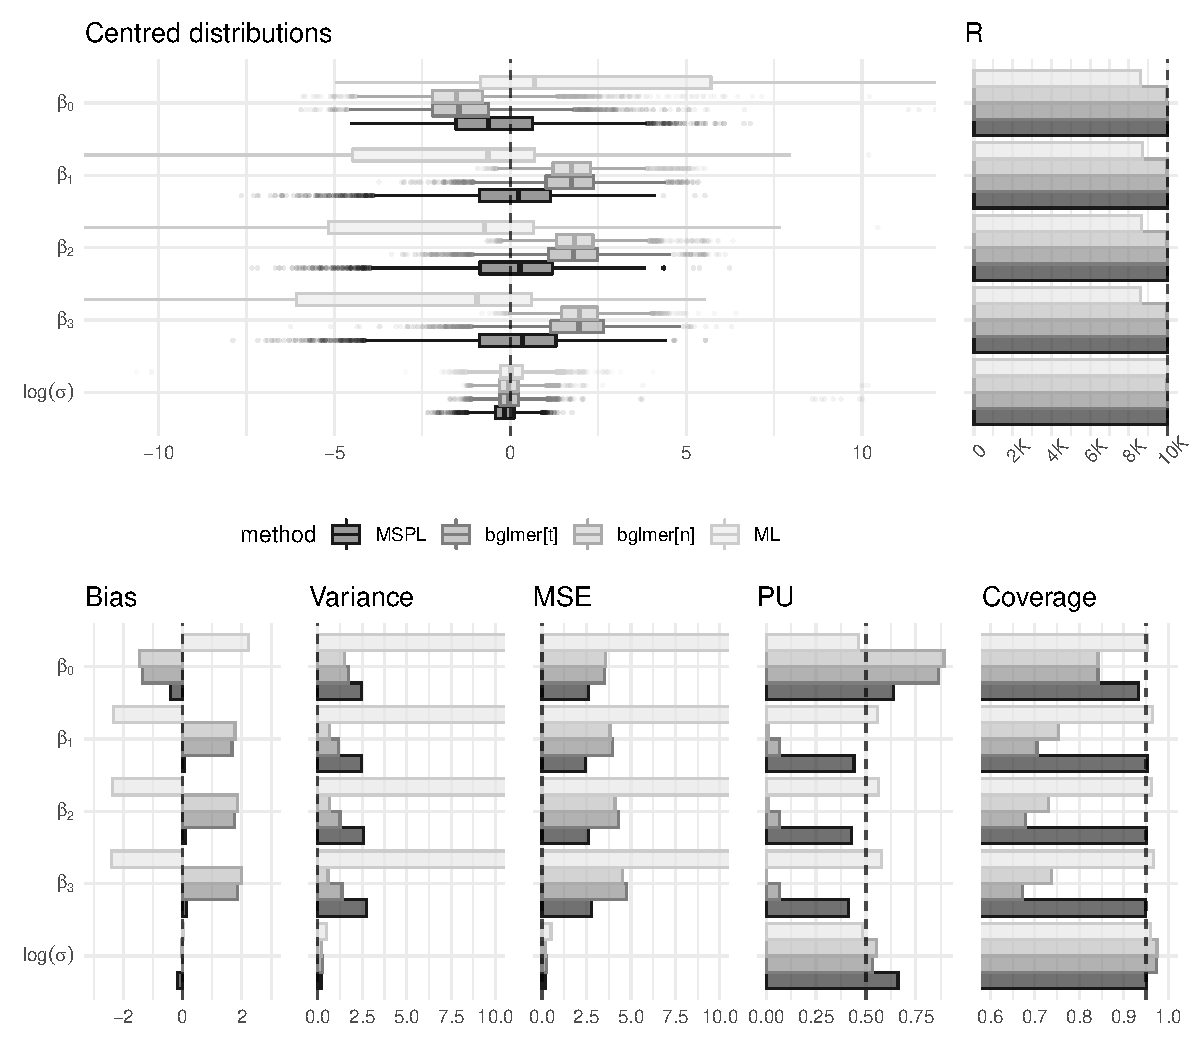
\includegraphics[width = \textwidth]{Figures/simulation_results.pdf}
  \end{center}
  \caption{Simulation results based on $10000$ simulated samples from \eqref{eq:logistic_normal} at the ML estimates in Table~S1 in the Supplementary Material. Estimates are obtained using ML, bglmer, and MSPL estimators, with a 100-point adaptive Gauss-Hermite quadrature approximation to the likelihood. Boundary parameter estimates are discarded for the calculation of the simulation summaries. The number of estimates used for the calculation of summaries is given in the top right panel (R). The top left panel shows the centred sampling distribution of the estimators for MSPL, bglmer and ML. The bottom panels give simulation-based estimates of the bias, variance, mean squared error (MSE), the probability of underestimation (PU) and the coverage based on 95\% Wald-confidence intervals (Coverage).}
  \label{fig:culcita_simu0}
\end{figure}

In order to assess the impact of shrinkage on the frequentist
properties of the estimators, we simulate $10000$ independent samples
of responses for the randomized complete block design in
Table~\ref{tab:culcita}, using the ML estimates in the $\bbeta$
parametrization when all data points are used as true values (see
Table~XXX \IK{fixme} of the Supplementary Material). For
each sample, we compute the ML and MSPL estimates, as well as the
bglmer estimates based on normal and t priors.
Figure~\ref{fig:culcita_simu0} shows boxplots for the sampling
distributions of the estimators, centred at the true values, the
estimated finite-sample bias, variance, mean squared error, and
probability of underestimation for each estimator, along with the
estimated coverage of 95\% Wald confidence intervals based on the
estimates and estimated standard errors from the negative Hessian of
the approximate log-likelihood at the estimates. The plotting range
for the support of the distributions has been restricted to
$(-11, 11)$, which does not contain all ML estimates in the
simulation study but contains all estimates for the other methods. We
should note here that apart from the estimated probability of
underestimation, estimates for the other summaries are not
well-defined for ML, because the probability of boundary estimates is
positive. In fact, there were issues with at least one of the ML
estimates for $9.25\%$ of the simulated samples. These issues are
either due to convergence failures or because the estimates or
estimated standard errors have been found to be atypically large in
absolute value. The displayed summaries for ML are computed based
only on estimates which have not been found to be
problematic. Clearly, the amount of shrinkage induced by the normal
and t priors is excessive. Although the resulting estimators have
small finite-sample variance (with the one based on normal priors
having the smallest), they have excessive finite-sample bias, which is
often at the order of the standard deviation.  The combination of
small variance and large bias results in large mean squared errors,
and the sampling distributions to be located far from the respective
true values, impacting first-order inferences; Wald-type confidence
intervals about the fixed effects are found to systematically
undercover the true parameter value. Finally, both bglmer[n] and
bglmer[t] do not appear to prevent extreme positive variance estimates.

As is apparent from Table~\ref{tab:culcita_inf}, the MSPL estimates
appear to be equivariant under contrasts; the identities between the
$\bbeta$ and $\bgamma$ parameterization of of the model holding
exactly with the proposed MSPL estimates with the observed small
deviations are attributed to rounding and the stopping criteria used
for the numerical optimization of the penalized
log-likelihood. Furthermore, from Figure~\ref{fig:culcita_simu0} we
see that the penalty we propose not only ensures that estimates are
away from the boundary of the parameter space, but its soft nature
leads to estimators that possess the good frequentist properties that
would be expected by the ML estimator had it not taken boundary
values.

\section{Composite penalty}\label{sec:composite_penalty}
We define a penalty for the log-likelihood or an approximation thereof 
for mixed effects logistic regression that returns MPL
estimators that are always in the interior of the parameter space and
are equivariant to scaled contrasts of the fixed-effects. The penalty
is appropriately scaled to be soft enough to return MPL
estimators that are consistent and asymptotically normally distributed. For this reason the
resulting MPL estimators are termed maximum
softly-penalized likelihood (MSPL) estimators.

Let $\btheta = (\bbeta^\top, \bpsi^\top)^\top$ and
$\ell(\btheta) = \log L(\bbeta, s(\bpsi))$ with $s(\bpsi) = \bSigma$,
where $L(\bbeta, s(\bpsi))$ is~\eqref{eq:bern_likl}. For clarity of presentation, we shall write $\ell(\btheta)$ to denote both the log-likelihood or an appropriate
approximation of the log-likelihood that is bounded from above. Sufficient conditions for consistency and asymptotic normality of the maximum softly penalized estimator under the exact model likelihood and an approximation thereof are provided in Section \ref{sec:softpen} of the Appendix. The parameter vector $\bpsi$ is defined as
$\bpsi = (\log l_{11}, \ldots, \log l_{qq}, l_{21}, \ldots, l_{q1},
l_{32}, \ldots, l_{q2}, \ldots, l_{qq-1})^\top$, where $l_{ij}$
$(i > j)$ is the $(i,j)$th element of the lower-triangular Cholesky factor $\bL$ of $\bSigma$, i.e.
$\bSigma = \bL\bL^\top$. Consider the estimator
\[
  \tilde{\btheta} = \arg\max_{\btheta \in \ \Theta} \left\{\ell(\btheta) + c_1 P_{(f)}(\bbeta) + c_2 P_{(v)}(\bpsi) \right\}\, ,
\]
where $c_{1} > 0$, $c_{2} > 0$, and $P_{(f)}(\bbeta)$ and
$P_{(v)}(\bpsi)$ are unscaled penalty functions for the fixed effects
and variance components, respectively. 

For the unscaled fixed effects penalty, we use the logarithm of
Jeffreys' invariant prior for the corresponding GLM, that is
\begin{equation}
  \label{eq:jeffreys_pen}
  P_{(f)}(\bbeta) = \frac{1}{2}\log \det\left(\sum_{i = 1}^k \bX^\top_i \bW_i \bX_i\right)\,,
\end{equation}
where $\bX_i$ collects the covariates for the fixed effects in
model~(\ref{eq:bern_cluster}), and $\bW_i$ is a diagonal matrix with
$j$th diagonal element $\mu_{ij}^{(f)} (1 - \mu_{ij}^{(f)})$ with
$\mu_{ij}^{(f)} = \exp(\eta_{ij}^{(f)}) / \{1 +
\exp(\eta_{ij}^{(f)})\}$ and $\eta_{ij}^{(f)} = \bx_{ij}^\top
\bbeta$. For the variance components penalty, we use a composition of
negative Huber loss functions on the components of $\bpsi$. In
particular,
\begin{equation}
  \label{eq:huber_pen}
  P_{(v)}(\bpsi) = \sum_{i = 1}^q D(\log l_{ii}) + \sum_{i > j} D(l_{ij}) \, ,
\end{equation}
where
\[
  D(x) = \begin{cases}
           -\frac{1}{2} x^2, & \text{if } |x|\leq 1 \\ 
           - |x| + \frac{1}{2}, & \text{otherwise}           
         \end{cases} \,.
\]

\section{Non-boundary MPL estimates}
\label{sec:non_boundary}

Denote by $\partial \Theta$ the boundary of $\Theta$ and let
$\btheta(r)$, $r \in \Re$, be a path in the parameter space such that
$\lim_{r \to \infty}\btheta(r) \in \partial \Theta$. A common approach
to resolving issues with ML estimates being in $\partial \Theta$, like
those encountered in the example of Section~\ref{sec:culcita_dat}, is
to introduce an additive penalty to the (approximate) log-likelihood
that satisfies $\lim_{r \to \infty} P(\btheta(r)) = -\infty$.  Hence,
if $\ell(\btheta)$ is bounded from above and there is at least one
point $\btheta \in \Theta$ such that
$\ell(\btheta) + P(\btheta) > -\infty$, then $\tilde\btheta$ is in the
interior of $\Theta$.

\citet[Theorem 1]{kosmidis+firth:2021} show that if the matrix $\bX$
with row blocks $\bX_1, \ldots, \bX_n$ is full rank, then the limit
of~(\ref{eq:jeffreys_pen}) is zero as $\bbeta$ diverges to any point
with at least one infinite component. This result holds for a range of
link functions including the commonly-used logit, probit,
complementary log-log, log-log and the cauchit link
\citep[see][Section~3.1, for details]{kosmidis+firth:2021}. Now,
noting that~\eqref{eq:bern_likl} is always bounded from above by one
as a probability mass function, the penalized log-likelihood
$\ell(\btheta) + P(\btheta)$ will diverge to $-\infty$ as $\bbeta$
diverges, for any value of $\bpsi$. Hence, the MPL estimates for the
fixed-effects always have finite components as long as there is at
least one point in $\Theta$ such that the penalized log-likelihood, or an approximation thereof,
is not $-\infty$. 

The penalty~\eqref{eq:huber_pen} on the variance
components takes value $-\infty$ whenever at least one component of
$\bpsi$ diverges.  Hence, by parallel arguments to those in the
previous paragraph, the penalized log-likelihood
$\ell(\btheta) + P(\btheta)$ will diverge to $-\infty$ as any
component of $\bpsi$ diverges, for any value of $\bbeta$. Hence, the
MPL estimates for $\bpsi$ have finite components and the value of
$\tilde\bSigma = s(\tilde{\bpsi})$ is guaranteed to be non-degenerate
in the sense that it is positive definite with finite entries, implying
correlations away from one in absolute value (see
Theorem~\ref{thm:nondeg}), as long as there is at least one point in
$\Theta$ such that the penalized log-likelihood is not $-\infty$.

The condition on the boundness of~\eqref{eq:bern_likl} is just on of
the sufficient conditions for the finiteness of the MPL estimates,
which is also satisfied by a vanilla (non-adaptive) Gauss-Hermite
quadrature or simulation-based approximations to the likelihood
\citep[see, for example,][]{mcculloch:1997}. A weaker sufficient
condition is that the penalized objective diverges to $-\infty$ as
$\btheta(r)$ diverges to $\partial \Theta$, or, in other words, that
the penalty dominates the likelihood in absolute value for any
divergent path. From the numerous numerical experiments we carried
out, we encounted no evidence that this weaker condition does not hold
for the adaptive quadrature and Laplace approximations to the
log-likelihood that the \texttt{glmer} routine of the R package
\texttt{lme4}.

The penalties arising from the independent normal and independent t
prior structures implemented in \texttt{blme} are such that
$\lim_{r \to \infty} P(\btheta(r)) = -\infty$, whenever $\btheta(r)$
diverges to the boundary of the parameter space for the fixed
effects. As a result, the bglmer[n] and bglmer[t] estimates for the
fixed effects are always finite, as also illustrated in
Table~\ref{tab:culcita_inf}. Nevertheless, the default gamma-prior
like penalty used in \texttt{bglmer} for the variance component
$\sigma$ is $-1.5 \log\sigma$, which, while it ensures that the
estimate of $\log \sigma$ is not minus infinity, does not guard from
positive infinite estimates. This is apparent in
Figure~\ref{fig:culcita_simu0}, where several extreme positive
bglmer[n] and bglmer[t] estimates are observed for $\log\sigma$.
% . see
% the analysis in Section~\ref{sec:ci} and the vignettes of the
% \texttt{glmmsr} \citep{ogden:2019} R package for an example with
% infinite variance component estimate in a Bernoulli-response GLMM
% \IK{Is this a mixed effects logistic regression?}\PS{this is with a probit link, the package has been removed from CRAN}.

\section{Equivariance under linear transformations of fixed effects}\label{sec:invariance}
The ML estimates are known to be equivariant under transformations of
the model parameters \citep[see, for example][]{zehna:1966}.  A
particularly useful class of transformations in mixed effects logistic
regression, and more generally GLMMs, with categorical covariates is
the collection of scaled linear transformations $\bbeta' = \bC \bbeta$
of the fixed effects for known, invertible, real matrices $\bC$.

Such invariance properties of the ML estimates guarantee that one can
obtain ML estimates and corresponding estimated standard errors for
arbitrary sets of scaled parameter contrasts of the fixed-effects,
when estimates for one of those sets of contrasts are available and
with no need to re-estimate the model. Such equivariance properties
eliminate any estimation and inferential ambiguity when two
independent researchers analyse the same data set using the same model
with different contrasts for the fixed effects, for example, due to
software defaults.

Following the argument in \citet{zehna:1966}, the
condition required for achieving equivariance of MPL estimators is that
the penalty for the fixed effects parameters behaves like the
log-likelihood under linear transformations; that is
\begin{equation}
  \label{eq:invariance}
  P_{(f)}(\bC\bbeta) = P_{(f)}(\bbeta) + a
\end{equation}
where $a \in \Re$ is a scalar that does not depend on $\bbeta$.

Let $\eta_{ij} = \bx_{ij}^\top \bC^{-1} \bgamma + \bz_{ij}^\top \bu_i$
in~\eqref{eq:bern_cluster} for a known real matrix $\bC$. Then,
$\bgamma = \bC\bbeta$, and the penalty for the fixed effects in the
$\bgamma$ parametrization is
$P_{(f)}(\bgamma) = P_{(f)}(\bbeta) - \log \det (\bC)$, which is of
the form~\eqref{eq:invariance}. In contrast, the penalties arising
from the normal and t prior structures used to compute the bglmer[n]
and bglmer[t] fixed effect estimates in Table~\ref{tab:culcita_inf} do
not satisfy~\eqref{eq:invariance}. Hence, the bglmer[n] and bglmer[t]
estimates are not equivariant under linear transformations of the
parameters.

\section{Consistency and asymptotic normality of the MSPL estimator}
\label{sec:asymptotics}
According to Theorem~\ref{thm:jeffrey_deriv_bound} in the Appendix
% on the bounds for the first-order partial
% derivative of the logarithm of the Jeffreys' invariant prior,
the gradient of the Jeffreys' invariant prior
in~\eqref{eq:jeffreys_pen} can be bounded as
$\vnorm{\nabla_{\bbeta} P_{(f)}(\bbeta)} \le p^{3/2} \max_{s,t}
|x_{st}|/2$, where $x_{st}$ is the $t$th element in the $s$th row of
$\bX$ as defined in Section \ref{sec:non_boundary}, where
$\vnorm{\cdot}$ is the Eucledian norm. Furthermore,
$\vnorm{\nabla_{\bpsi} P_{(v)}(\bpsi)} \le \sqrt{q(q+1)/2}$ because
$|d D(x) / dx| \le 1$. Hence, an application of the triangle
inequality gives that
$\vnorm{\nabla_{\btheta} P(\btheta)} \le c_1 p^{3/2} \max_{s, t}
|x_{st}| / 2 + c_2 \sqrt{q(q+1) / 2}$. For the scaling factors $c_1$
and $c_2$, we propose using $c_1 = c_2 = c$ to be the square root of
the average of the approximate variances of $\hat\eta_{ij}^{(f)}$ at
$\bbeta = \b0_p$. A delta method argument gives that
$c = 2 \sqrt{p/n}$. Therefore,
\[
\vnorm{\nabla_{\btheta} P(\btheta)} \le \frac{p^{2}}{\sqrt{n}} \max_{s, t} |x_{st}|  +  \sqrt{\frac{2pq(q+1)}{n}} \, .
\]
Hence, $\delta^\infty = o_p(r_n)$, and the conditions on
$\delta^\infty$ in Theorem~\ref{thm:soft_pen_cons} and
Theorem~\ref{thm:asymp_norm_soft_pen} are satisfied, as long as
$\max_{s, t} |x_{st}| = O_p(n^{1/2})$. The condition on the maximum of
the absolute elements of the model matrix is not unreasonable in
practice. It certainly holds true for covariates such as dummy
variables, as included in the real-data examples in the current
paper. It is also true for model matrices with subgaussian random
variables with common variance proxy $\sigma^2$, in which case
$\max_{s,t} |x_{st} | = \Op{\sqrt{2\sigma^2 \log(2np)}}$ \citep[see,
for example,][Theorem 1.14]{rigollet:2015}.

\section{Conditional inference data} 
\label{sec:ci}
To demonstrate the performance of the MSPL on a Bernoulli-response
GLMM with multivariate random effects structure, we consider a subset
of the data analysed by \citet{singmann+etal:2016}. As discussed on
CrossValidated
(\url{https://stats.stackexchange.com/questions/38493}), this data set
exhibits both infinite fixed effects estimates as well as degenerate
variance components estimates when a Bernoulli-response GLMM is fitted
by ML.
	
The data set, originally collected as a control condition of experiment 3)b) in \citet{singmann+etal:2016} and therein analysed in a different context, comes from an experiment in which participants worked on a probabilistic conditional inference task. Participants were presented with the conditional inferences modus ponens (MP; ``\textit{If p then q. p. Therefore q.}''), modus tollens (MT; ``\textit{If p then q. Not q. Therefore  not p.}''), affirmation of the consequent (AC; ``\textit{If p then q. q. Therefore p}''), and denial of the antecedent (DA, ``\textit{If p then q. Not p. Therefore not q}''), and asked to estimate the probability that the conclusion (``\textit{Therefore ...}'') follows from the conditional rule (``\textit{If p then q.}'') and the minor premise (``\textit{p, not p, q, not q}.''). The material of the experiment consisted of the following four conditional rules with varying degrees of counterexamples (alternatives, disablers; indicated in parentheses below).
\begin{enumerate}
\item If a predator is hungry, then it will search for prey. (few disablers, few alternatives)
\item If a person drinks a lot of coke, then the person will gain weight. (many disablers, many alternatives)
\item If a girl has sexual intercourse with her partner, then she will get pregnant. (many disablers, few alternatives)
\item If a balloon is pricked with a needle, then it will quickly lose air. (few disablers, many alternatives)
\end{enumerate}
To illustrate, for MP and conditional rule 1, a participant was asked: ``\textit{If a predator is hungry, then it will search for prey. A predator is hungry. How likely is it that the predator will search for prey?}'' Additionally, participants were asked to estimate the probability of the conditional rule, e.g. ``\textit{How likely is it that if a predator is hungry it will search for prey?}'', and the probability of the minor premises, e.g. ``\textit{How likely is it that a predator is hungry?}''. 
	
The response variable of this data set is then a binary response indicating whether, given a certain conditional rule, the participants' probabilistic inference is $p$-valid. An inference is deemed $p$-valid, if the summed uncertainty of the premises does not exceed the uncertainty of the conclusion, where uncertainty of a statement $x$ is defined as one minus the probability of $x$. For example, for MP, a respondent's inference is $p$-valid if $1-\Pr(\textit{``q''}) \leq 1 - \Pr(\textit{``Ìf p then q''}) + 1-\Pr(\textit{``p''}) $, where $\Pr(x)$ indicates the participant's estimated probability of statement $x$ ($p$-valid inferences are recorded as zero, $p$-invalid inferences as one). Covariates are the categorical variable ``counterexamples'' (``many'', ``few''), that indicates the degree of available counterexamples to a conditional rule, ``type'' (``affirmative'',``denial'') which describes the type of inference (MP and AC are affirmative, MT and DA are denial), and ``$p$-validity'' (``valid'',``invalid''), indicating whether an inference is $p$-valid in standard probability theory where premise and conclusions are seen as events (MP and MT are $p$-valid, while AC and DA are not). For each of the 29 participants, there exist 16 observations corresponding to all possible combinations of inference and conditional rule, giving a total of 464 observations, which are grouped along individuals by the clustering variable ``code''. We can employ a Bernoulli-response GLMM to investigate the probabilistic validity of conditional inference given the type of inference and conditional rule as captured by the covariates and all possible interactions thereof. We introduce a random intercept and random slope for the variable counterexamples to account for response heterogeneity between participants. Hence the model we are considering is given by    
\begin{align}
  \label{eq:cond_inf_model} 
  Y_{ij} \mid \bb{u}_i & \sim \text{Bernoulli}(\mu_{ij}) \quad \text{with} \quad
                         g(\mu_{ij}) = \eta_{ij} = \bx_{ij}^\top \bbeta + \bz_{ij}^\top \bu_i\\
  \bu_i & \sim \text{N}(\b0_2, \bb{\Sigma})  \quad (i = 1, \ldots, 29; j = 1, \ldots, 16)\,,
\end{align}
where $\bbeta = (\beta_0,\beta_1,\ldots,\beta_8)$ are the fixed effects pertaining to the model matrix of the R model formula \texttt{response \raisebox{-0.9ex}{\~{}} type * p.validity * counterexamples + (1+counterexamples|code)}. As (adaptive) Gauss-Hermite quadrature becomes computationally challenging and not available for \texttt{glmer} and consequently \texttt{bglmer} for multivariate random effect structures, we approximate the likelihood of model \eqref{eq:cond_inf_model} about the parameters $\bbeta$, $\bL$ using Laplace's method (see for example \cite{pinheiro+bates:1995}). We estimate the parameters $\bbeta$, $\bL$ by ML using the optimization routines CG (ML[CG]) and BFGS (ML[BFGS]) of the \texttt{optimx} R package \citep{nash:2014}, \texttt{bglmer} from the \texttt{blme} R package \cite{chung+etal:2013} using independent normal (bglmer[n]) and t (bglmer[t]) priors for the fixed effects and the default Wishart prior for the multivariate variance components. We also estimate the parameters using the proposed MSPL estimator with the fixed and random effects penalties of Section \ref{sec:composite_penalty}. The estimates are given in Table \ref{tab:cond_inf}, where we denote the entries of $\bL$ by $l_{st}$, for $s,t=1,2$. 
\begin{table}[t]
  \centering
 \caption{ML, bglmer and MSPL estimates for the parameters of model~\eqref{eq:cond_inf_model} using a Laplace approximation to the log-likelihood. Estimated standard errors (in parentheses) are based on the negative Hessian of the approximate likelihood. A $-$ indicates that the estimated standard error could not be computed due to floating point overflow.}
 \label{tab:cond_inf}
  \centering
  \begin{tabular}{lrrrrrr}
    \toprule
    &
      \multicolumn{1}{c}{ML[BFGS]} & 
			\multicolumn{1}{c}{ML[CG]} &
			\multicolumn{1}{c}{bglmer[t]} &
			\multicolumn{1}{c}{bglmer[n]} & 
			\multicolumn{1}{c}{MSPL} \\
			\midrule
			$\beta_0$ & 16.28 & 7.63 & 10.60 & 10.04 & 6.22 \\ 
			& (2.09) & (3.69) & (1.56) & (1.23) & (2.49) \\ 
			$\beta_2$ & 4.27 & 3.22 & 1.57 & 1.28 & 0.00 \\ 
			& (4.57) & (14.94) & (1.58) & (1.80) & (2.83) \\ 
			$\beta_3$ & -6.75 & -2.08 & 0.12 & 0.35 & -2.17 \\ 
			& (3.02) & (5.19) & (1.59) & (1.40) & (2.60) \\ 
			$\beta_4$ & -14.44 & -5.80 & -8.50 & -7.90 & -4.37 \\ 
			& (2.13) & (3.75) & (1.80) & (1.35) & (2.51) \\ 
			$\beta_5$ & 3.21 & 0.85 & 0.41 & 0.45 & 2.17 \\ 
			& (3.34) & (16.63) & ($-$) & (0.35) & (4.07) \\ 
			$\beta_6$ & -4.27 & -3.24 & -1.70 & -1.45 & 0.00 \\ 
			& (4.60) & (14.95) & (1.62) & (1.92) & (2.86) \\ 
			$\beta_7$ & 8.25 & 3.78 & 1.16 & 0.86 & 3.64 \\ 
			& (3.13) & (5.26) & (1.77) & (1.63) & (2.71) \\ 
			$\beta_8$ & -3.94 & -1.81 & -0.89 & -0.86 & -2.87 \\ 
			& (3.49) & (16.67) & ($-$) & (1.29) & (4.18) \\ 
			$\log l_{1,1}$ & 2.02 & 0.73 & 3.34 & 3.34 & -0.63 \\ 
			& (0.16) & (1.03) & (0.00) & (0.01) & (2.48) \\ 
			$l_{2,1}$ & -7.67 & -2.25 & -28.35 & -28.13 & -0.60 \\ 
			& (0.97) & (2.29) & (0.12) & ($-$) & (1.69) \\ 
			$\log l_{2,2}$ & -5.17 & -2.92 & -0.65 & -0.73 & -1.21 \\ 
			& (83.15) & (8.01) & (0.75) & (0.83) & (1.30) \\ 
			\bottomrule
  \end{tabular}
\end{table}
As in the Culcita example of Section \ref{sec:culcita_dat}, we encounter fixed effects estimates that are extreme on the logistic scale for ML[BFGS], ML[CG] and bglmer[t]. We further note that the strongly negative estimates for $l_{22}$ in conjunction with the inflated asymptotic standard errors of the ML[BFGS] estimates are highly indicative of parameter estimates on the boundary of the parameter space, meaning that $l_{22}$ is essentially estimated as zero. The degeneracy of the variance components estimates is even more striking for the bglmer estimates, which give estimates of $l_{11},l_{21}$ greater than $28$ in absolute value, which corresponds to estimated variance components greater than $800$ in absolute value. This underlines that, as with the gamma prior penalty for univariate random effects, the Wishart prior penalty, while effective in preventing variance components being estimated as zero, cannot guard against infinite estimates for the variance components. We finally note that for the MSPL, all parameter estimates as well as their estimated standard errors appear to be finite. Further, while the variance components penalty guards against estimates that are effectively zero, the penalty induced shrinkage towards zero is not as strong as with the Wishart prior penalty of the \texttt{bglmer} function. 

To further investigate the frequentist properties of the estimators on this data set, we repeat the simulation design of the Culcita data example from Section \ref{sec:culcita_dat} for the conditional inference data at the MSPL estimate of Table \ref{tab:cond_inf}. We point out the extremely low percentage of bglmer estimates without estimation issues that were used in the summary of Figure \ref{fig:cond_inf_simul}. We note that the MSPL %,which is the only estimation method that is guaranteed to give non-degenerate variance components estimates, 
outperforms ML and bglmer, which incur substantial bias and variance due to their singular and infinite variance components estimates. Table \ref{tab:cond_inf}, which shows the percentiles of the centred estimates for each estimator, shows that ML and \texttt{bglmer} return heavily distorted variance components estimates, reflecting the fact that these estimators are unable to fully guard against degenerate variance components estimates. A comprehensive simulation summary for all parameters is given in Figure~S1 and Table~S2 of the Supplementary Material. 

\begin{figure}[ht]
  \begin{center}
    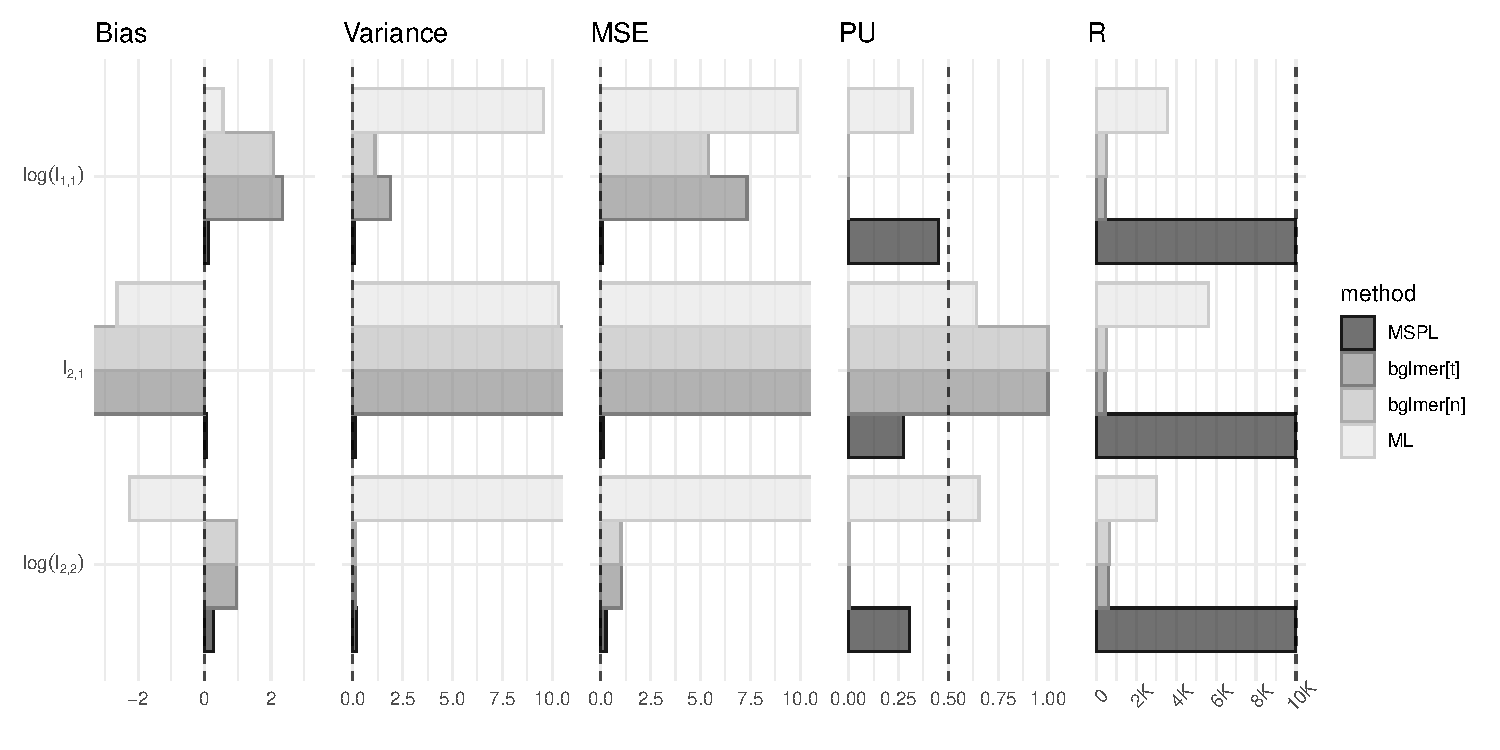
\includegraphics[width=\textwidth]{Figures/cond_inf_simul.pdf}
  \end{center}
  \caption{Simulation based estimates of the bias, variance, mean squared-error (MSE), and the probability of underestimation (PU), for MSPL, bglmer and ML estimators based on $10000$ simulated samples from~\eqref{eq:cond_inf_model} at the MSPL estimates in Table~\ref{tab:cond_inf}. Boundary estimates were discarded for the calculation of the simulation summaries. The number of samples used for the calculation of summaries per parameter is given in the rightmost panel (R).
  }\label{fig:cond_inf_simul}
\end{figure}

\begin{table}[H]
  \centering
  \caption{Percentiles of centred variance components estimates from simulating samples from model~(\ref{eq:cond_inf_model}) at the MSPL of Table~\ref{tab:cond_inf}.} 
  \label{tab:sim2}
  \begin{tabular}{lrccccccc}
	 \toprule 
	&& \multicolumn{7}{c}{Percentiles} \\ \cmidrule{3-9} 
	&&$5\%$&$10\%$&$25\%$&$50\%$&$75\%$&$90\%$&$95\%$\\ \cmidrule{3-9} 
	\cmidrule{3-9} 
	& $\log l_{1,1}$ & -0.06 & -0.05 & -0.02 & 0.01 & 0.12 & 0.44 & 0.66 \\ 
	MSPL & $l_{2,1}$ & -0.66 & -0.27 & -0.02 & 0.12 & 0.21 & 0.35 & 0.45 \\ 
	& $\log l_{2,2}$ & -0.42 & -0.31 & -0.08 & 0.26 & 0.58 & 0.87 & 1.02 \\ 
	\cmidrule{3-9} 
	& $\log l_{1,1}$ & 0.95 & 1.04 & 1.21 & 1.91 & 3.81 & 4.55 & 4.92 \\ 
	bglmer[t] & $l_{2,1}$ & -38.54 & -34.65 & -4.03 & -2.73 & -1.29 & -0.92 & -0.78 \\ 
	& $\log l_{2,2}$ & 0.44 & 0.58 & 0.74 & 0.95 & 1.16 & 1.36 & 1.52 \\ 
	\cmidrule{3-9} 
	& $\log l_{1,1}$ & 1.05 & 1.19 & 1.40 & 1.80 & 2.04 & 4.23 & 4.60 \\ 
	bglmer[n] & $l_{2,1}$ & -39.24 & -34.03 & -3.87 & -2.86 & -1.63 & -1.06 & -0.84 \\ 
	& $\log l_{2,2}$ & 0.43 & 0.55 & 0.73 & 0.94 & 1.16 & 1.36 & 1.51 \\ 
	\cmidrule{3-9} 
	& $\log l_{1,1}$ & -2.75 & -2.05 & -0.91 & 1.21 & 2.36 & 2.62 & 2.66 \\ 
	ML & $l_{2,1}$ & -7.47 & -7.19 & -5.74 & -1.51 & 0.54 & 0.81 & 1.09 \\ 
	& $\log l_{2,2}$ & -6.62 & -4.54 & -3.22 & -1.77 & 0.39 & 0.85 & 1.04 \\ 
	\bottomrule 
  	\bottomrule 
  \end{tabular}
\end{table}

\section{Concluding remarks}
\label{sec:sum}
This paper proposed the MSPL estimator for stable parameter estimation
in mixed effects logistic regression models. The method has been
found, both theoretically and empirically, to have superior finite
sample properties to the maximum penalized estimator proposed in
\citet{chung+etal:2013}. We showed that penalizing the model
log-likelihood by scaled versions of the Jeffreys' prior for the model
with no random effects and of a composition of the negative Huber loss
for the variance components gives estimates in the interior of the
parameter space and that appropriate scaling of the penalty function
preserves the optimal ML asymptotics, namely consistency, asymptotic
normality and Cram\'{e}r-Rao efficiency.

We note here that the conditions of Theorem~\ref{thm:soft_pen_cons}
and Theorem~\ref{thm:asymp_norm_soft_pen} that are used for
establishing the consistency and asymptotic normality of the MSPL
estimator in Section~\ref{sec:asymptotics} are merely sufficient;
there may be other sets of conditions that lead to the same results.

While the MSPL is particularly relevant for mixed effects logistic
regression, the concept is far more general and we expect it to be
useful in other settings, for which degenerate ML estimates are known
to occur, such as generalized linear mixed models (GLMMs) with
categorical or ordinal responses. In particular, the composite
negative Huber loss penalty can readily applied to other GLMMs, to
prevent singular variance components estimates. We point out that the
bound on the partial derivations of the Jeffreys' prior in
Theorem~\ref{thm:jeffrey_deriv_bound} for a logistic GLM extends to
the cauchit link up to a constant; bounds for other link functions,
like the probit and the complementary log-log are the subject of
current work.

\section{Supplementary Materials}
The supplementary material to this paper, which is available at \url{https://github.com/psterzinger/softpen_supplementary}, consists of the four folders ``Scripts'', ``Data'', ``Results'', ``Documents'' and a readme file. ``Scripts'' contains all scripts to recreate the numerical analyses, simulations, graphics and tables of the paper. ``Data'' contains the datasets used in Sections \ref{sec:culcita_dat} and \ref{sec:ci}, and ``Result'' stores all results pertaining to these anylises and to the examples in the Supplementary Material. ``Documents'' contains the tex files of the paper, a supplementary material document, with further material to the examples and simulations and
additional simulation studies and the relevant figures and bibliography. All numerical results are exactly replicable in R version 4.2.0 (2022-04-22), and with the following packages: blme~1.0-5 \citep{chung+etal:2013}, doMC~1.3.8 \citep{doMC}, dplyr~1.0.9 \citep{dplyr}, lme4~1.1-29 \citep{bates+etal:2015}, MASS~7.3-56 \citep{MASS}, numDeriv~2016.8-1.1 \citep{gilbert+varadhan:2019}, optimx~2022-4.30 \citep{nash:2014}. Dependent packages and packages that are not essential for the replication of the numerical results are not listed in the interest of brevity.
\appendix

\section{Theorem~\ref{thm:nondeg}}

\begin{theorem}
  \label{thm:nondeg}
  Let $\tilde{\bb L} \in \Re^{q \times q}$ be a real, lower triangular matrix with finite entries and strictly positive entries on its main diagonal. Then $\tilde{\bb \Sigma} = \tilde{\bb L}\tilde{\bb L}^\top$ is not degenerate. 
\end{theorem}
\begin{proof}
	Recall that a variance-covariance matrix is not degenerate if it is positive definite with finite entries, implying correlations away from one in absolute value. We prove each property in turn. To see that $\tilde{\bb \Sigma}$ is positive-definite, take any $\bb x\in \Re^q:\bb x\neq \bb 0_q$. Then by straightforward manipulations 
      %   \begin{equation}
      %   \label{eq:chol1}
      %   \begin{aligned}
      %   \bb x^\top\tilde{\bb \Sigma}\bb x &= \bb x^\top\tilde{\bb L}\tilde{\bb L}^\top\bb x\\ 
      %   &= (\tilde{\bb L}^\top\bb x)^\top\tilde{\bb L}^\top\bb x \\ 
      %   &= \langle \bb y,\bb y\rangle, \quad \bb y=\tilde{\bb L}^\top\bb x\\
      %   &\geq 0
      %   \end{aligned}
      % \end{equation}
        \begin{equation}
          \label{eq:chol1}
        \bb x^\top\tilde{\bb \Sigma}\bb x = \bb x^\top\tilde{\bb L}\tilde{\bb L}^\top\bb x
	= (\tilde{\bb L}^\top\bb x)^\top\tilde{\bb L}^\top\bb x 
	= \langle \tilde{\bb L}^\top\bb x, \tilde{\bb L}^\top\bb x\rangle \geq 0
      \end{equation}
      where $\langle\cdot,\cdot\rangle$ denotes the standard Euclidean inner product. Hence $\tilde{\bb \Sigma}$ is positive semidefinite. Suppose that there is some $\bb x \in \Re^d$ such that $\bb x^\top \bb \Sigma \bb x=0$. Then by \eqref{eq:chol1}, $\langle \tilde{\bb L}^\top\bb y, \tilde{\bb L}^\top\bb y \rangle = 0$ which holds if and only if $\tilde{\bb L}^\top\bb y=\bb 0_d$. Now since $\tilde{\bb L}$ is lower triangular with strictly positive diagonal entries, it is full rank. %To see this, assume that $\tilde{\bb L}\bb x=\bb 0_d$ and note that $[\tilde{\bb L}\bb x]_1 = l_{11}x_1$. Since $\tilde{l}_{11}>0$, it must be that $x_1=0$. Now $[\tilde{\bb L}\bb x]_2 = \tilde{l}_{21}x_1+\tilde{l}_{22}x_2$. Since $x_1=0$ and $\tilde{l}_{22}>0$ it must again hold that $x_2=0$ and by induction $\bb x=\bb 0_d$ so that $\tilde{\bb L}$ is full rank.
	But then $\bb y = \tilde{\bb L}^\top \bb x=\bb 0_d$ implies that $\bb x = \bb 0_d$ so that $\tilde{\bb \Sigma}$ is positive definite. 
	To prove that $\tilde{\bb \Sigma}$ has finite entries, note that $\tilde{\bb \Sigma}_{st} = \langle \tilde{\bb l}_s,\tilde{\bb l}_t \rangle$, where $\tilde{\bb l}_s$ is the $s$th row vector of $\tilde{\bb L}$. Since all elements of $\tilde{\bb l}_s,\tilde{\bb l}_t$ are finite, so is their inner product.  
	Finally, towards a contradiction, assume that $\tilde{\bb \Sigma}$ implies correlations of one in absolute value. Then there exist indices $s,t, s \neq t$ such that 
	% \begin{alignat}{2}\label{eq:chol2}
	% &\qquad& 
	% \left|\frac{\tilde{\bb \Sigma}_{st} }{\sqrt{ \tilde{\bb \Sigma}_{ss} \tilde{\bb \Sigma}_{tt}}}\right|&=1 \\ 
	% \iff&& |\tilde{\bb \Sigma}_{st}| &= \sqrt{ \tilde{\bb \Sigma}_{ss} \tilde{\bb \Sigma}_{tt}} \\ 
	% \iff && |\langle \tilde{\bb l}_s,\tilde{\bb l}_t\rangle| &= \|\tilde{\bb l}_s\|\|\tilde{\bb l}_t\|\label{eq:chol3}
	% \end{alignat}
        \[
          \left|\frac{\tilde{\bb \Sigma}_{st} }{\sqrt{ \tilde{\bb \Sigma}_{ss} \tilde{\bb \Sigma}_{tt}}}\right| =1 	\iff |\tilde{\bb \Sigma}_{st}| = \sqrt{ \tilde{\bb \Sigma}_{ss} \tilde{\bb \Sigma}_{tt}}  
	\iff |\langle \tilde{\bb l}_s,\tilde{\bb l}_t\rangle| = \|\tilde{\bb l}_s\|\|\tilde{\bb l}_t\|
        \]
	where $\|\bb x\|= \sqrt{\langle\bb x ,\bb x\rangle}$ is the induced inner product norm. It follows from the Cauchy-Schwarz inequality that the last equality holds if and only if $\tilde{\bb l}_s,\tilde{\bb l}_t$ are linearly dependent. Since $\tilde{\bb L}$ is lower triangular, this is only possible if $\tilde{\bb l}_s,\tilde{\bb l}_t$ have zeros in the same positions. But since all diagonal entries of $\tilde{\bb L}$ are strictly positive, this is not possible.
\end{proof}

\section{Consistency and asymptotic normality of MPL estimators}
\label{sec:softpen}

\subsection{Setup}

Suppose that we observe the values $\by_1, \ldots, \by_k$ of a
sequence of random vectors $\bY_1, \ldots, \bY_k$ with
$\by_i = (y_{i1}, \ldots, y_{in_i})^\top \in \mathcal{Y} \subset
\Re^{n_i}$, possibly with a sequence of covariate vectors
$\bv_1, \ldots, \bv_k$, with
$\bv_i = (v_{i1}, \ldots, v_{is})^\top \in \mathcal{X} \subset
\Re^{s}$. Let $\bY = (\bY_1^\top, \ldots, \bY_k^\top)^\top$, and
denote by $\bV$ the set of $\bv_1, \ldots, \bv_k$. Further, assume
that the data generating process of $\bY$ conditional on $\bV$ has a
density or probability mass function $f(\bY \mid \bV; \btheta)$,
indexed by a parameter $\btheta \in \Theta \subset \Re^d$. Denote the
parameter that identifies the conditional distribution of $\bY$ given
$\bV$ by $\btnod \in \Theta$.

Define the ML estimator as
$\hat\btheta = \arg \max_{\btheta\in \Theta} \ell(\btheta)$, where
$\ell(\btheta) = \log f(\bY \mid \bV; \btheta)$, and let
$\tilde\btheta$ be the MPL estimator
$\tilde\btheta = \arg\max_{\btheta \in \Theta}\{\ell(\btheta) +
P(\btheta) \}$, where $P(\btheta)$ is an additive penalty to
$\ell(\btheta)$ that may depend on $\bY$ and $\bV$. Consistency and
asymptotic normality of the proposed MPL estimator follow readily from
similar such results for ML estimators in \citet{ogden:2017} where the
approximation error to the model log-likelihood is an additive error
term. In fact, the results presented in this section are a direct
translation of the work in \citet{ogden:2017}, where the term
``approximation error'' is replaced by ``penalty function''.

\subsection{Consistency}

The consistency of $\bttilde$ can be established under the following
regularity conditions on the log-likelihood gradient
\citep[see][Chapter 5]{vaart:1998} and the penalty gradient.
	\begin{itemize}
	\item[A1] $\ell(\btheta)$ is differentiable with gradient
          $S(\btheta)$.
	\item[A2]
          $\underset{\btheta \in \Theta}{\sup} \; \vnorm{r_n^{-1}
            S(\btheta) - S_0(\btheta)} \overset{p}{\to}0$ for some
          deterministic function $S_0(\btheta)$ for some increasing
          sequence $\{r_n\}$.
	\item[A3] For all $\varepsilon>0$,
          $\underset{\btheta \in \Theta: \vnorm{\btheta-\btnod}\geq
            \varepsilon}{\inf} \vnorm{S_0(\btheta) }>0 =
          \vnorm{S_0(\btnod)}$.
        \item[A4] $P(\btheta)$ is differentiable with gradient $A(\btheta)$.
        \end{itemize}
       
      	Define $\hat{\btheta}$ and $\tilde{\btheta}$ to be such that
        $S(\hat{\btheta}) = \b0_d$ and
        $S(\tilde{\btheta}) + A(\tilde{\btheta}) = \b0_d$,
        respectively.  Furthermore, let
        $\delta(\btheta) = \vnorm{A(\btheta)}$ for some vector norm
        $\vnorm{\cdot}$, and, for $S \subseteq \Theta$, define
        $\delta^\infty(S) = {\sup}_{\btheta \in S} \; \delta(\btheta)$
        and let $\delta^\infty = \delta^\infty(\Theta)$.

        
        \begin{theorem}[Consistency]
          \label{thm:soft_pen_cons}
          Suppose that A1-A4 hold and $\delta^\infty = o_p(r_n)$. Then, $\bttilde \overset{p}{\to} \btnod$.
        \end{theorem}

        \begin{proof}
          The proof is analogous to the proof of \citet[Theorem
          1]{ogden:2017} and follows from
          \citet[Theorem~5.9]{vaart:1998} on the consistency of
          $M$-estimators. \citet[Theorem~5.9]{vaart:1998} states that
          under assumptions A2 and A3 about the log-likelihood
          gradient, if $r_n^{-1}S(\bttilde) = o_p(1)$ then
          $\bttilde \overset{p}{\to} \btnod$. It holds that
          \begin{equation}
            \label{eq:soft_pen_cons_proof_1}
              \vnorm{ r_n^{-1}S(\bttilde) } = \vnorm{ r_n^{-1}\left\{S(\bttilde) + A(\bttilde)\right\} - r_n^{-1}A(\bttilde) }
                                           = \vnorm{ \b0_d- r_n^{-1}  A(\bttilde) } 
                                           = o_p(1) \, .
          \end{equation}
          The second equality follows from the definition of
          $\tilde\btheta$, and the last equality follows from the
          assumption that $\delta^\infty = o_p(r_n)$.
          % So, $\tilde\btheta$ is consistent.
        \end{proof}          
        
        \subsection{Asymptotic normality}

        The asymptotic normality of $\bttilde$ can be established under the
        following conditions
        % (e.g. \citep[Section 3]{hbe4} \PS{no ref?}).
        
        \begin{itemize}
	\item[A5] $\ell(\btheta)$ is three times differentiable.
	\item[A6]
          $\sup_{\btheta \in \Theta} \mnorm{r_n^{-1}J(\btheta)
            -I(\btheta) } \overset{p}{\to} 0$ for some positive
          definite $O(1)$ matrix $I(\btheta)$, that is continuous in
          $\btheta$ in a neighbourhood around $\btnod$, for some
          increasing sequence $\{r_n\}$.
	\item[A7]
          $r_n^{1/2}(\hat\btheta-\btnod) \overset{d}{\to}
          \text{N}(0,I(\btnod)^{-1})$.
	\item[A8] $\bttilde \overset{p}{\to} \btnod$.
        \item[A9] $P(\btheta)$ is three times differentiable.
        \end{itemize}
        
%        It is assumed that the information about $\btheta$ accumulates
%        at a rate $r_n$ in the sense that
%        $r_n^{-1}J(\btheta ) \overset{p}{\to} I(\btheta)$ as
%        $n \to \infty$ for some nonrandom, positive definite, $O(1)$
%        matrix $I(\btheta)$ and with respect to some matrix norm,
%        where $J(\btheta) = -\nabla \nabla^\top \ell(\btheta)$ is the
%        observed information matrix.
       
\begin{theorem}[Asymptotic Normality]
  \label{thm:asymp_norm_soft_pen}
  Suppose that A5-A9 hold and that $\delta^\infty = o_p(r_n^{1/2})$. Then, $r_n^{1/2}(\bttilde-\btnod) \overset{d}{\to} \text{N}(0,I(\btnod)^{-1})$.
\end{theorem}
\begin{proof}
	We show that $\tilde{\bb \theta} -\hat{\bb \theta} = o_p(r_n^{-1/2})$, which, by A7, establishes the claim. Let $S(\btheta)$ be the gradient of $\ell(\btheta)$ and $J(\btheta) = -\nabla\nabla^\top \ell(\btheta)$ and consider a first-order Taylor expansion of $r_n^{-1}S(\btheta)$ around $\hat{\btheta}$. 
	\begin{equation}\label{eq:norm_taylor}
	r_n^{-1}S(\btheta) = r_n^{-1}S(\hat{\btheta}) + r_n^{-1} \nabla S(\btheta^*) (\btheta-\hat{\btheta}) = \b0_q -J(\btheta^*)(\btheta-\hat{\btheta})
	\end{equation}
	where $\btheta^*$ lies between $\btheta$ and $\hat{\btheta}$ and the second equality follows by the definition of $\hat{\btheta}$ and $J(\btheta)$. Hence
	\begin{equation}\label{eq:norm_taylor2}
	\b0_q = r_n^{-1}S(\bttilde) + r_n^{-1}A(\bttilde) = r_n^{-1} A(\bttilde) - r_n^{-1}J(\btheta^*)(\bttilde-\hat{\btheta})  \, , 
	\end{equation}
	where the first equality follows by the definition of $\bttilde$ and the second from substituting the RHS of \eqref{eq:norm_taylor} for $S(\bttilde)$. Therefore 
	\begin{equation}
	\tilde{\bb \theta} -\hat{\bb \theta} = [r_n^{-1}J(\btheta^*)]^{-1} [r_n^{-1}A(\bttilde)] \, . 
	\end{equation}
	By A6, and an application of the continuous mapping theorem (see for example \citet[Theorem 2.1]{vaart:1998}), $[r_n^{-1}J(\btheta^*)]^{-1} = \Op{1}$ and since $\delta^\infty = o_p(r_n^{1/2})$ by assumption, $r_n^{-1}A(\bttilde) = o_p(r_n^{-1/2})$. Therefore $\tilde{\bb \theta} -\hat{\bb \theta} = o_p(r_n^{-1/2})$ as required. 
\end{proof}

\subsection{Approximate likelihoods}

We note that the large sample results for the MPL estimator derived
here operate under the assumption that $\ell(\btheta)$ is the exact
model log-likelihood. If $\bar{\ell}(\btheta)$ is an approximation to
the exact log-likelihood then consistency and asymptotic normality can
be established under extra conditions on
$\bar\delta^\infty = \sup_{\btheta \in \Theta}\vnorm{ \bar{S}(\btheta)
  - S(\btheta) }$, where $\bar{S}(\btheta)$ is the gradient of
$\ell(\btheta)$. In particular, for consistency it is sufficient that
$\bar\delta^\infty = o_p(r_n)$, and for asymptotic normality it is
sufficient that $\bar{\ell}(\btheta)$ is three-times differentiable
and $\bar\delta^\infty = o_p(r_n^{1/2})$. In this instance, one can
replace all occurrences of $A(\btheta)$ by
$A(\btheta) + \bar{S}(\btheta)-S(\btheta)$ in the proofs of Theorems
\ref{thm:soft_pen_cons} and \ref{thm:asymp_norm_soft_pen}. A simple
application of the triangle inequality establishes that
$\underset{\btheta \in \Theta}{\sup} \vnorm{A(\btheta) +
  \bar{S}(\btheta)-S(\btheta)}$ is of the same stochastic order as
$\delta^\infty$ in the assumptions of the Theorems and thus the proofs
apply.

% There are results on approximation errors of the log-likelihhod,
% that can be adapted to match our conditions.
We refer the reader to \citet{ogden:2021} for approximation errors to
the log-likelihood in clustered GLMMs using Laplace's method,
\citet{ogden:2017} for approximation errors to the gradient of the
log-likelihood with an example for an intercept-only
Bernoulli-response GLMM, \citet{stringer:2022} for approximation
errors to the log-likelihood in clustered GLMMs using Adaptive
Gauss-Hermite quadrature and \citet{jin+andersson:2020} for general
approximation errors for adaptive Gauss-Hermite quadrature.

\section{Bound on the gradient of the logarithm of the Jeffreys' prior}
\begin{theorem}[Bound on the partial derivative of the log of Jeffreys'  prior]\label{thm:jeffrey_deriv_bound}
	Let $\bb X $ be the $n\times p$ full column rank matrix defined in Section \ref{sec:non_boundary}, and $\bb W$ a block-diagonal matrix with blocks $\bW_i$ as defined in Section \ref{sec:composite_penalty} ($i=1,\ldots,k$). Then 
\[        
  \left|\frac{\partial }{\partial  \beta_s}\log \det(\bb X^\top\bb W\bb X)\right| \leq p\underset{1\leq t\leq n}{\max} |x_{ts}|, 
\]
where $x_{ts}$ denotes the $t$th element in the $s$th column of $\bX$.
\end{theorem}
\begin{proof}
	We shall find it notationally convenient to neglect the block-structure of $\bX$ and refer to the $t$th element of the $s$th column of $\bX$ by $x_{ts}$ and define $\mu_t^{(f)}(\bbeta) = \exp(\eta_t^{(f)}(\bbeta))/(1+\exp(\eta_t^{(f)}(\bbeta)))$ for $\eta_t^{(f)}(\bbeta) = \bx_t^\top\bbeta$, and where $\bx_t^\top$ is the $t$th row of $\bX$. It is noted without proof that 
\[
	\left|\frac{\partial }{\partial \beta_s}\log \textrm{det}(\bb X^\top\bb W\bb X)\right|  = \text{tr}\left( (\bb X^\top\bb W\bb X)^{-1}\bb X^\top\bb W\widetilde{\bb W}_s\bb X \right)
\]
	where $\widetilde{\bb W}_s$ is a diagonal matrix with main-diagonal entries $\widetilde{w}^{(s)}_{t}= x_{ts}(1-2\mu_t^{(f)}(\bb\beta))$. 
	Now by the cyclical property of the trace, it follows that 
\[
	\text{tr}\left( (\bb X^\top\bb W\bb X)^{-1}\bb X^\top\bb W\widetilde{\bb W}_s\bb X \right) =\text{tr}\left( \bb X(\bb X^\top\bb W\bb X)^{-1}\bb X^\top\bb W\widetilde{\bb W}_s \right)
\]
	For notational brevity, denote the projection matrix $\bb X(\bb X^\top\bb W\bb X)^{-1}\bb X^\top\bb W$ by $\bb P$. Since $\widetilde{\bb W}_s$ is a diagonal matrix, one gets that 
	\begin{align*} 
	\left| \text{tr}\left( \bb X(\bb X^\top\bb W\bb X)^{-1}\bb X^\top\bb W\widetilde{\bb W}_s \right) \right| &=  \left| \sum_{t=1}^{n}\widetilde{w}_t^{(s)}[\bb P]_{tt} \right| \\ 
	&\leq \sum_{t=1}^{n}\left|\widetilde{w}_t^{(s)}[\bb P]_{tt} \right| \\ 
	&= \sum_{t=1}^{n}\left|\widetilde{w}_t^{(s)}\right|[\bb P]_{tt}  \\ 
	&\leq \underset{1\leq t \leq n}{\max}\; \left|\widetilde{w}_t^{(s)}\right| \sum_{t=1}^{n}[\bb P]_{tt}  \\ 
	%		&= \underset{1\leq j \leq n}{\max}\; \left|\widetilde{w}_j^{(i)}\right| \sum_{j=1}^{n}\lambda_j(\bb P)\\ 
	&=p \underset{1\leq t \leq n}{\max}\; \left|\widetilde{w}_t^{(s)}\right|\\ 
	&=p \underset{1\leq t \leq n}{\max}\; \left|x_{ts}(1-2\mu_t^{(f)}(\bb\beta))\right| \\ 
	&\leq p\underset{1\leq t \leq n}{\max}\;\left|x_{ts}\right|  
	\end{align*}
	Here the second line is due to the triangle inequality. The third line follows by nonnegativity of the main-diagonal elements of $\bb P$. To see this, note that $\bb X^\top\bb W\bb X$ is positive definite as $\bb X$ has full column rank and $\bb W$ is a diagonal matrix with positive entries. It thus follows that $(\bb X^\top\bb W\bb X)^{-1}$ is positive definite. Hence for any $\bb y \in \Re^{n}, \|\bb y\|_2\neq 0$, $\bb y^\top\bb X(\bb X^\top\bb W\bb X)^{-1}\bb X \bb y = \tilde{\bb y}^\top(\bb X^\top\bb W\bb X)^{-1} \tilde{\bb y} \geq 0$, for $\tilde{\by} = \bX \by$, so that $\bb X(\bb X^\top\bb W\bb X)^{-1}\bb X$ is positive semi-definite. It is well known that the main diagonal entries of a positive semi-definite matrix are nonnegative. Hence, as $\bb W$ is a diagonal matrix with nonnegative diagonal entries it follows that the main diagonal entries of $\bb P$, which are the elementwise product of the diagonals of $\bb X(\bb X^\top\bb W\bb X)^{-1}\bb X$ and $\bb W$ are nonnegative. The fifth line follows since $\bb P$ is an idempotent matrix of rank $p$, and the fact that the trace of an idempotent matrix equals its rank \citep[Corollary 10.2.2]{harville:1998}. The fact that $\bb P$ has rank $p$ follows from the assumption that $\bb X$ has full column rank and since $\bb W$ is invertible for any $\bb\beta \in \Re^p,\bb X\in \Re^{n \times p}$ by construction and is a standard result in linear algebra (see for example \cite{magnus+neudecker:2019}, Chapter 1.7).  The last line follows since $\mu_t^{(f)}(\bb\beta) \in (0,1)$. 
	
\end{proof}	



\bibliographystyle{chicago}
\bibliography{softpen}

% 
\includepdf[pages=-]{softpen_supplementary.pdf}
\end{document}
